\documentclass[italian]{article}

\usepackage{amsmath}
\usepackage{babel}
\usepackage{booktabs}
\usepackage{boxedminipage}
\usepackage{graphics}
\usepackage{pgfplotstable}

\begin{document}

\section{Clustering}

	Clustering é suddividere un dataset di un certo numero di elementi
	in sottoparti chiamate cluster sulla base della loro affinitá.

	Il problema é che diversi algoritmi di clustering non sono in grado di
	fornire una metrica oggettiva per determinare quanto il clustering che
	hanno indotto sia effettivamente rappresentativo della struttura del
	dataset, o se sia semplicemente un raggruppamento arbitrario. Inoltre,
	diversi algoritmi come K-Means richiedono il numero di cluster come
	iperparametro, rendendo il discorso ancora piú complesso, perché in
	genere nel clustering non supervisionato non vi é a disposizione
	alcuna "ground truth".

	La metrica Silhouette si propone di rispondere alle seguenti domande:

	\begin{itemize}
		\item
		Il clustering è di buona qualitá? In altre parole, gli elementi di
		uno stesso cluster sono fra di loro "vicini" ed al contempo "lontani"
		dagli elementi di tutti gli altri cluster?
		\item
		Quali sono gli elementi ben classificati, ovvero quelli che probabilmente
		si trovano nel cluster "giusto"?
		\item
		Quali sono gli elementi che é difficile stabilire con certezza in quali
		cluster vadano collocati, ovvero quelli che stanno "nel mezzo" fra piú
		cluster?
		\item
		Il numero di cluster scelto é effettivamente rappresentativo del dataset
		o è 'artificioso'?
	\end{itemize}

\section{Silhouette}

	\subsection{Setup}

		Si supponga di avere a disposizione un dataset di dimensione
		$N times M$, dove $N$ indica il numero degli elementi e $M$ é
		il numero di attributi. Per comoditá, si assuma che gli attributi
		siano tutti dati numerici (altezze, lunghezze, capacitá, ecc...).
		Per ogni elemento, tutti i valori di ciascun attributo sono noti.

		A partire da tale dataset é possibile costruire quella che viene
		chiamata \textbf{matrice delle distanze}. Tale matrice ha dimensione
		$N \times N$ e, in ciascuna cella $(i, j)$, é presente un valore
		indicato con $d(i, j)$ che rappresenta il grado di "dissomiglianza"
		fra l'elemento $i$ e l'elemento $j$ del dataset.

		Tale grado di dissomiglianza é calcolato mediante una
		\textbf{funzione di distanza}, usando come input i valori
		degli attributi di $i$ e di $j$. Un esempio di funzione di
		distanza é la \textbf{distanza Euclidea}, definita come segue:

		\begin{equation}
			d(i, j) =
			\sqrt{\sum_{m = 1}^{M} (f_{i, m} - f_{j, m})^{2}} =
			\sqrt{(f_{i, 1} - f_{j, 1})^{2} + \dots +
			      (f_{i, M} - f_{j, M})^{2}}
		\end{equation}

		Dove $f_{i, m}$ e $f_{j, m}$ indicano il valore del $m$-esimo
		attributo per, rispettivamente, l'$i$-esimo ed il $j$-esimo
		elemento del dataset.

		Altri esempi di distanze sono la \textbf{distanza di Manhattan}
		e la \textbf{distanza di Minkowski} (dal punto di vista di
		Silhouette, quale funzione di distanza venga usata é irrilevante).

		\begin{table}[h]
			\centering
			\pgfplotstabletypeset[
				col sep=comma,
				header=true,
				every head row/.style={before row=\toprule, after row=\midrule},
				every last row/.style={after row=\bottomrule},
				]{data/dist.csv}
			\caption{Matrice delle distanze per il dataset \texttt{iris}. Per questioni
			di spazio sono presenti solamente i primi 6 elementi.}
			\label{tab:dist}
		\end{table}

		Una volta nota la matrice delle distanze, si supponga di applicare
		un algoritmo di clustering (K-Means, ad esempio) per suddividere il
		dataset in un certo numero di cluster, sia questo $K$. Per ciascun
		cluster, é interamente noto sia il numero di suoi elementi, sia
		a quale cluster ciascun elemento del dataset é stato assegnato.

	\subsection{Costruzione di $a(i)$ e $b(i)$}

		Per poter calcolare il coefficiente di Silhouette, é prima necessario
		introdurre due quantitá per ciascun elemento $i$ del dataset, indicate
		rispettivamente con $a(i)$ e $b(i)$.

		Preso un elemento $i$ del dataset, sia $A$ il cluster in cui l'algoritmo
		lo ha riposto. Ammesso che $A$ contenga altri elementi all'infuori di $i$,
		é possibile definire $a(i)$ come distanza media fra $i$ e tutti gli elementi
		di $A$ escluso $i$ stesso:

		\begin{equation}
			a(i) = \frac{1}{|A| - 1} \sum_{j \in \{A - \{i\}\}} d(i, j)
		\end{equation}

		Tale valore misura quanto un cluster é \textit{coeso}, nel senso
		che se tale valore é piccolo per tutti gli elementi del cluster,
		questi si trovano fra loro vicini. Per tale motivo, $a(i)$ viene
		anche chiamata \textbf{distanza intra-cluster}.

		Dopodiché, in maniera simile, per un cluster $C$ diverso da $A$
		è possibile definire $D(i, C)$ come la distanza media fra $i$
		(che appartiene ad $A$) e gli elementi di $C$:

		\begin{equation*}
			D(i, C) = \frac{1}{|C|} \sum_{j \in C} d(i, j)
		\end{equation*}

		Tale valore misura quanto un cluster é \textit{separato}, nel senso
		che se tale valore é grande per tutti gli elementi del cluster a cui
		$i$ appartiene, il cluster nel suo complesso si trova molto distante
		da tutti gli altri. Per tale motivo $D(i, C)$ viene anche chiamata
		\textbf{distanza inter-cluster}.

		Assumendo che il numero di cluster sia piú di uno, per uno stesso elemento
		$i$ é possibile calcolare la distanza inter-cluster per ogni possibile
		cluster $C$ distinto da $A$. Fra questi $K - 1$ cluster, é di particolare
		interesse il cluster che ha il piú piccolo valore di distanza inter-cluster
		per $i$, chiamato \textbf{neighboring cluster}. Questo perché tale cluster
		é quello che, se il cluster $A$ non esistesse, sarebbe la miglior scelta
		per catalogare $i$, dato che é quello i cui elementi sono i piú vicini ad
		$i$.

		Se il neighboring cluster per $i$ é il cluster $C'$, la distanza
		inter-cluster $D(i, C')$ viene indicata con $b(i)$:

		\begin{equation}
			b(i) = min_{C \neq A} D(i, C)
		\end{equation}

	\subsection{Calcolo di $s(i)$}

		Una volta calcolato $a(i)$ e $b(i)$ per l'elemento $i$ del dataset, é
		possibile assegnarvi un valore di Silhouette $s(i)$, cosí calcolato:

		\begin{equation}
			s(i) = \frac{b(i) - a(i)}{max\{a(i), b(i)\}}
		\end{equation}

		Se l'elemento $i$ si trova in un cluster che contiene solamente sé stesso,
		per convenzione il valore $s(i)$ viene posto a $0$ (é una scelta arbitraria,
		ma é anche quella piú neutra).

		É facile verificare che, per qualsiasi elemento $i$:

		\begin{equation*}
			-1 \leq s(i) \leq 1
		\end{equation*}

		Si assuma infatti che $b(i) \geq a(i)$. L'espressione diventa:

		\begin{equation*}
			s(i) = \frac{b(i) - a(i)}{b(i)} =
			\frac{b(i)}{b(i)} - \frac{a(i)}{b(i)} =
			- \frac{a(i)}{b(i)}
		\end{equation*}

		Avendo assunto che $b(i)$ sia maggiore di $a(i)$, tale frazione é una
		frazione propria, e pertanto il suo valore é racchiuso nell'intervallo
		$[-1, 0]$.

		Si assuma invece $a(i) > b(i)$. L'espressione diventa:

		\begin{equation*}
			s(i) = \frac{b(i) - a(i)}{a(i)} =
			\frac{b(i)}{a(i)} - \frac{a(i)}{a(i)} =
			\frac{b(i)}{a(i)}
		\end{equation*}

		Avendo assunto che $a(i)$ sia maggiore di $b(i)$, tale frazione é una
		frazione propria, e pertanto il suo valore é racchiuso nell'intervallo
		$[0, 1]$.

		%Inoltre, $s(i)$ non varia se tutte le distanze vengono moltiplicate
		%per una costante $q$:
		%
		%\begin{equation*}
		%	s(i) = \frac{m b(i) - m a(i)}{max\{m a(i), m b(i)\}} =
		%	\frac{m(b(i) - a(i))}{m(max\{a(i), b(i)\})} =
		%	\frac{b(i) - a(i)}{max\{a(i), b(i)\}}
		%\end{equation*}

		\begin{table}
			\begin{boxedminipage}{0.25\linewidth}
					\pgfplotstabletypeset[
						col sep=comma,
						header=true,
						every head row/.style={before row=\toprule, after row=\midrule},
						every last row/.style={after row=\bottomrule},
					]{data/siOne.csv}
			\end{boxedminipage}
			\begin{boxedminipage}{0.25\linewidth}
					\pgfplotstabletypeset[
						col sep=comma,
						header=true,
						every head row/.style={before row=\toprule, after row=\midrule},
						every last row/.style={after row=\bottomrule},
					]{data/siTwo.csv}
			\end{boxedminipage}
			\begin{boxedminipage}{0.25\linewidth}
					\pgfplotstabletypeset[
						col sep=comma,
						header=true,
						every head row/.style={before row=\toprule, after row=\midrule},
						every last row/.style={after row=\bottomrule},
					]{data/siThree.csv}
			\end{boxedminipage}
			\caption{Valori di $s(i)$, cluster e neighboring cluster per
			i primi 10 elementi dei tre cluster. Si noti come i valori
			di $s(i)$ del primo cluster siano piú alti ed il neighboring
			cluster sia sempre lo stesso, mentre gli altri due cluster
			hanno valori piú variegati.}
			\label{tab:iris}
		\end{table}

		Per farsi una migliore idea del significato di $s(i)$, puó essere
		utile considerare alcune situazioni estreme.

		Quando $s(i)$ è approssimativamente $1$ si ha che $b(i)$ é molto
		piú grande di $a(i)$, e quindi la distanza fra $i$ ed i membri del
		cluster a cui appartiene è molto piú piccola della distanza fra $i$
		ed i membri degli altri cluster. Questo significa che la scelta di
		aver posto $i$ in quel cluster é una buona scelta, perché persino
		la "seconda scelta" è di netto inferiore alla prima.

		Quando $s(i)$ é approssimativamente $0$ si ha che $b(i)$ e $a(i)$
		hanno lo stesso ordine di grandezza, e quindi la distanza fra $i$
		ed i membri del cluster a cui appartiene è comparabile a quella
		fra $i$ ed i membri del suo neighboring cluster. Questo significa
		che la scelta di aver posto $i$ in quel cluster è inconclusiva,
		nel senso che se fosse stato invece scelto il neighboring cluster
		si avrebbe avuto sostanzialmente lo stesso risultato.

		Quando $s(i)$ è approssimativamente $-1$ significa che $a(i)$ é molto
		piú grande di $b(i)$, e quindi la distanza fra $i$ ed i membri del
		cluster a cui appartiene é molto piú grande della distanza fra $i$
		ed i membri degli altri cluster. Questo significa che la scelta di
		aver posto $i$ in quel cluster é discutibile, perché vi sono cluster
		con cui $i$ ha piú in comune rispetto a quello in cui si trova.

		%Altra interessante proprietà: spostando i nel suo neighboring cluster
		%il valore di $s(i)$ cambia di segno. Questo perché, molto banalmente,
		%le distanze rimangono le stesse ma i ruoli di $a(i)$ e $b(i)$ si invertono.

	\subsection{Silhouette Plot}

		I valori $s(i)$ non sono, di per loro, particolarmente informativi.
		É peró possibile costruire un Silhouette plot di ciascun cluster
		come un bar chart dove ciascuna colonna $i$-esima ha altezza
		proporzionale a $s(i)$, ordinato dalla colonna piú alta a quella
		piú bassa. Tale grafico puó essere arricchito riportando informazioni
		ulteriori per ciascun elemento come, ad esempio: in quale cluster si
		trova, qual'é il suo neighboring cluster, il suo valore di $s(i)$.

		\begin{figure}
			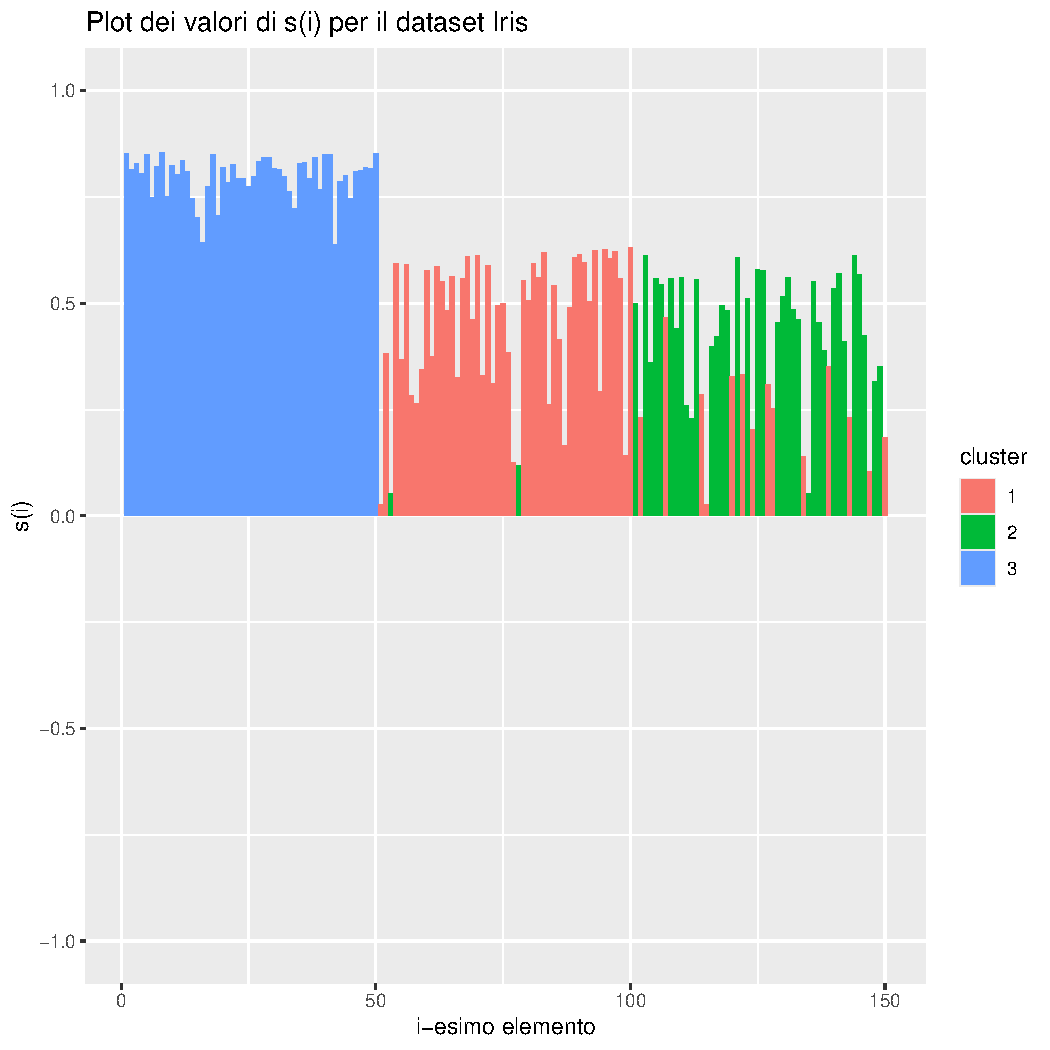
\includegraphics[width = \textwidth]{doc/si.pdf}
			\caption{Silhouette plot per il dataset \texttt{iris}.}
			\label{fig:si}
		\end{figure}

	\subsection{Come interpretare Silhouette}

		Il vantaggio di Silhouette é che non dipende da quale algoritmo
		é stato usato per effettuare il clustering. Per tale motivo, puó
		essere usato per valutare "a posteriori" il risultato dell'algoritmo,
		provando a modificare il valore degli iperparametri per valutare
		quale combinazione di iperparametri restituisce il risultato piú
		coerente. Questo riesce particolarmente bene negli algoritmi in
		cui il numero di cluster figura fra gli iperparametri, come K-Means.

		Per esempio, si supponga che un dataset abbia effettivamente
		delle aree molto dense separate da aree ampie vuote. Operando
		un clustering in cui il numero di cluster é piú basso del numero
		"naturale" di cluster, delle aree molto distanti tra loro vengono
		inglobate in un cluster unico nonostante vi siano considerevoli
		distanze nel mezzo. Silhouette può evidenziare questa situazione
		perché il valore di $a(i)$ tende ad essere molto alto, essendo
		i membri del dataset molto distanti dai loro centroidi.

		Si supponga invece di operare un clustering in cui il numero
		di cluster é piú alto del numero "naturale" di cluster. In tale
		situazione, anche aree dense vengono spezzate in cluster diversi.
		Silhouette può evidenziare questa situazione perché il valore di
		$b(i)$ tende ad essere molto basso, dato che elementi molto vicini
		vengono separati forzosamente.

		In generale, l'operato di un algoritmo di clustering puó
		considerarsi ottimale se il valore si $s(i)$ tende ad essere
		molto alto per tutti gli elementi del dataset. A tale scopo,
		é possibile calcolare la Silhouette media per un certo cluster
		$C$ come la media tutti gli $s(i)$ per ciascun elemento $i$
		che appartiene a $C$. Se tale valore medio é alto, il cluster
		nel suo complesso é ben formato.

		Se si ha invece interesse a sapere qual'é il numero ottimale di
		cluster, é possibile considerare la Silhouette media complessiva
		come la media di tutti gli $s(i)$ per ogni elemento dell'intero
		dataset. L'idea é quella di testare diverse combinazioni di
		iperparametri dell'algoritmo di clustering e scegliere la
		combinazione che restituisce la Silhouette media complessiva piú
		grande: tale combinazione sará quella che restituisce il clustering
		che meglio interpreta il dataset.

		\begin{figure}
			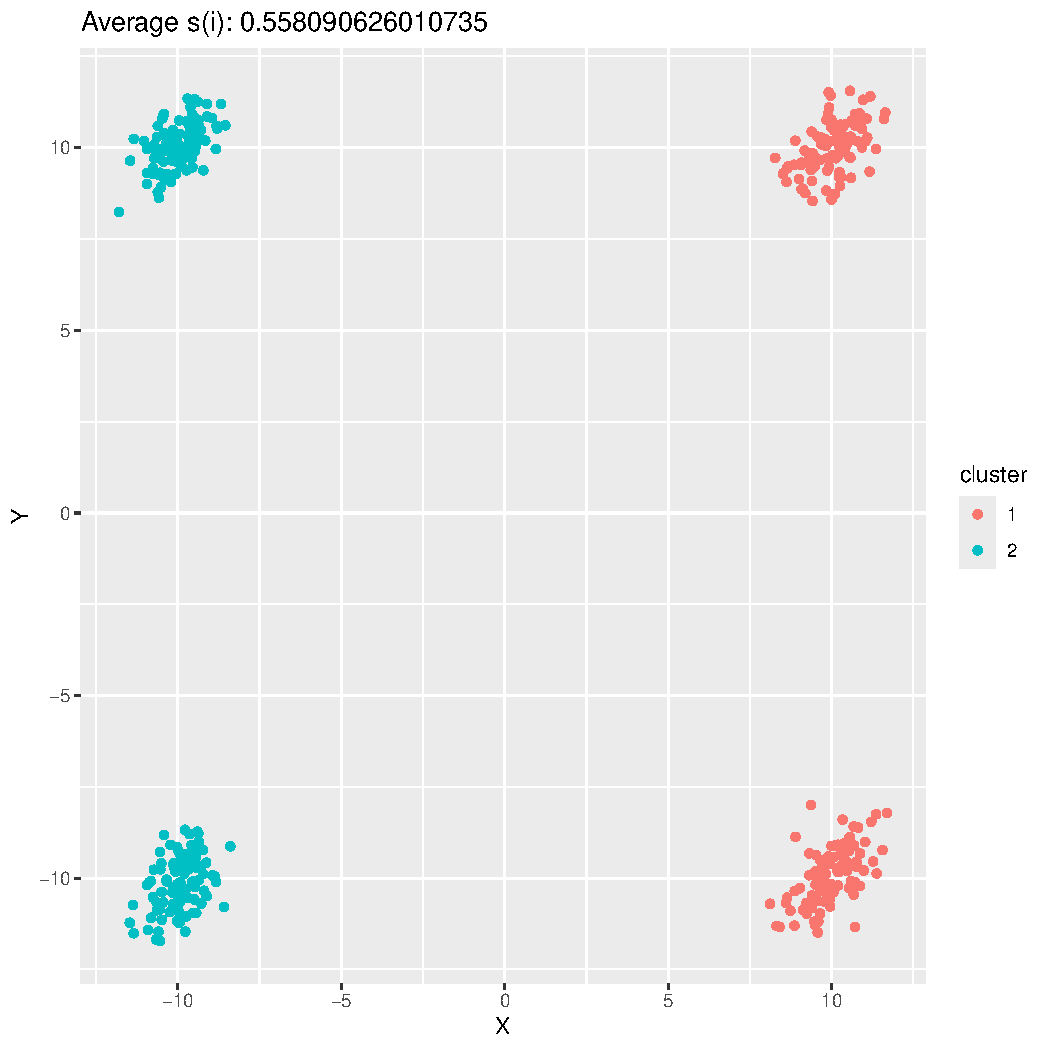
\includegraphics[width = \textwidth]{doc/clusters-2.pdf}
			\caption{Clustering con K-Means usando K = 2 per un dataset
			autogenerato in cui la struttura di cluster é ben visibile. }
			\label{fig:c2}
		\end{figure}

		\begin{figure}
			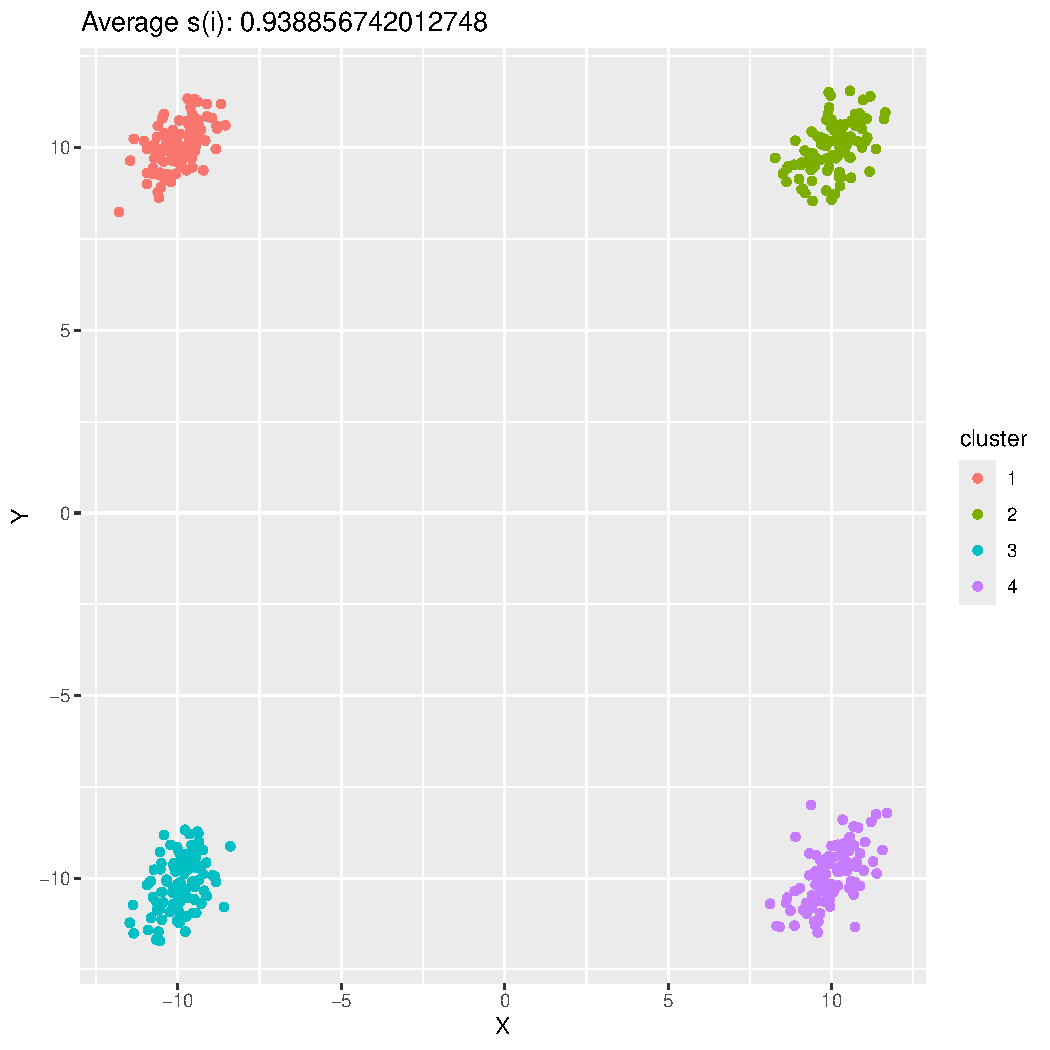
\includegraphics[width = \textwidth]{doc/clusters-4.pdf}
			\caption{Clustering con K-Means usando K = 4 per un dataset
			autogenerato in cui la struttura di cluster é ben visibile. }
			\label{fig:c4}
		\end{figure}

		\begin{figure}
			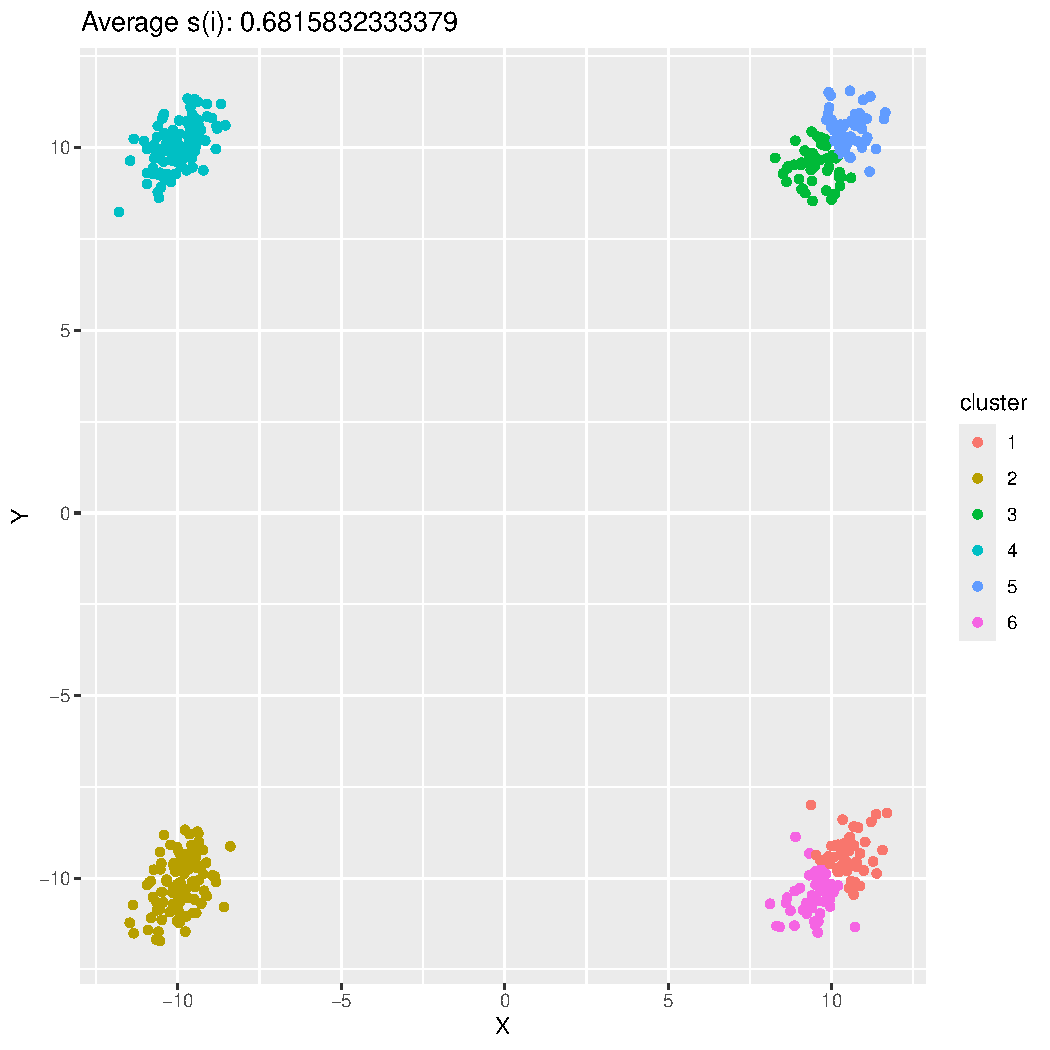
\includegraphics[width = \textwidth]{doc/clusters-6.pdf}
			\caption{Clustering con K-Means usando K = 6 per un dataset
			autogenerato in cui la struttura di cluster é ben visibile. }
			\label{fig:c6}
		\end{figure}

		Si noti come un valore della Silhouette media complessiva
		pari a $0$ non significa necessariamente che il clustering
		non sia andato a buon fine. Puó infatti anche indicare che
		effettivamente il dataset non ha alcuna struttura di clustering
		naturale, e che quindi l'algoritmo di clustering ha comunque
		fornito un risultato corretto, dato che effettivamente qualsiasi
		risultato vale l'altro.

	\subsection{Sviluppi futuri}

		A partire dall'idea di base di Silhouette, è possibile costruirne
		infinite varianti. Gli autori citano:

		\begin{itemize}
			\item
			Per determinare il miglior numero di cluster non è strettamente
			necessario utilizzare la Silhouette media complessiva. Sarebbe
			infatti possibile anche combinare gli $s(i)$ in modo diverso;
			\item
			La Silhouette media complessiva può essere essa stessa usata
			come funzione obiettivo da massimizzare direttamente all'interno
			di un algoritmo di clustering, anziché effettuare una valutazione
			a posteriori;
			\item
			Se l'algoritmo di clustering si basa sulla costruzione di centroidi
			o sulla elezione di rappresentanti, si potrebbe usare la distanza
			da tali centroidi o rappresentanti come grado di dissomiglianza
			anziché calcolare $a(i)$ o $D(i, C)$ per ogni $i$-esimo elemento,
			semplificando il procedimento. Naturalmente, questo approccio
			renderebbe Silhouette dipendente dal tipo di algoritmo usato. 
		\end{itemize}

		Tutte e tre le varianti sono toccate da articoli citati.

\end{document}
